% =============================================================================
% First-Year Progression Review -- presentation
% Flavio Gualtieri
% Compile with pdfLaTeX.
% =============================================================================
\documentclass[aspectratio=169,10pt]{beamer}

\usepackage[T1]{fontenc}
\IfFileExists{lmodern.sty}{\usepackage{lmodern}}{}
\usepackage{amsmath,amssymb}
\usepackage{ifthen}
\usepackage{adjustbox}
\usepackage{booktabs}
\usepackage{graphicx}
\usepackage{tikz}
\usepackage{pgfplots}
\pgfplotsset{compat=1.18}
\usetikzlibrary{positioning,arrows.meta,fit,backgrounds,calc,decorations.pathreplacing}

\graphicspath{{figs/}}

% ---------- look & feel (classic LaTeX) ----------------------
\usetheme{default}
\usecolortheme{default}
\setbeamertemplate{navigation symbols}{}
\setbeamerfont{frametitle}{size=\large,series=\bfseries}
\setbeamercolor{frametitle}{fg=black}
\setbeamertemplate{frametitle}{\vspace{0.30cm}\insertframetitle\vspace{-0.15cm}}
\setbeamertemplate{footline}{\hfill\scriptsize\color{gray}\insertframenumber\hspace{0.4cm}\vspace{0.15cm}}
\setbeamertemplate{itemize items}[triangle]
\setbeamercolor{itemize item}{fg=black}
\setbeamercolor{itemize subitem}{fg=black}
\setbeamercolor{enumerate item}{fg=black}

% ---------- palette ------------------------------------------
\definecolor{cblue}{HTML}{2E9FD6}
\definecolor{cgreen}{HTML}{16A085}
\definecolor{cpurple}{HTML}{A400C0}
\definecolor{corange}{HTML}{E8622A}
\definecolor{cred}{HTML}{E8192C}
\definecolor{cgray}{HTML}{555555}
\definecolor{cgood}{HTML}{16A085}
\definecolor{cbad}{HTML}{E8622A}

\pgfplotsset{
  barlegend/.style={
    legend image code/.code={\draw[#1] (0cm,-0.075cm) rectangle (0.3cm,0.075cm);}},
}

% ---------- block styles -------------------------------------
\tikzset{
  blk/.style   ={draw=none,text=white,font=\ttfamily\scriptsize,
                 minimum width=1.9cm,minimum height=0.42cm,inner sep=1pt},
  conv/.style  ={blk,fill=cblue},
  pool/.style  ={blk,fill=cgreen},
  lin/.style   ={blk,fill=cpurple},
  norm/.style  ={blk,fill=corange},
  tens/.style  ={font=\scriptsize,text=cred},
  note/.style  ={font=\scriptsize,text=cgray},
  arr/.style   ={-{Latex[length=2mm]},thick,cgray},
  box/.style   ={draw=cgray,thick,rounded corners=1pt,inner sep=2pt},
}

% full-height diagrams
\newenvironment{fitpic}
  {\begin{adjustbox}{max width=\textwidth,max totalheight=0.74\textheight,center}\begin{tikzpicture}}
  {\end{tikzpicture}\end{adjustbox}}
% compact diagrams -- use whenever there is body text under the picture
\newenvironment{fitpicS}
  {\begin{adjustbox}{max width=0.92\textwidth,max totalheight=0.42\textheight,center}\begin{tikzpicture}}
  {\end{tikzpicture}\end{adjustbox}}

% ---------- reusable pictures (from pi_multik_prez.tex) ------
\newcommand{\pointcloud}[1]{%
\begin{scope}[shift={#1}]
 \foreach \x/\y in {0.20/1.05,0.32/1.22,0.15/0.90,0.38/0.98,0.26/0.78,
                    0.55/1.30,0.62/1.12,0.48/1.42,
                    0.95/0.62,1.08/0.75,0.88/0.48,1.15/0.55,1.02/0.38,0.80/0.68,
                    1.45/1.05,1.58/1.18,1.38/0.90,1.62/0.95,1.50/1.28,
                    1.72/0.35,1.85/0.48,1.95/0.28,1.78/0.18,2.02/0.45}
   {\fill[black] (\x,\y) circle (0.035);}
\end{scope}}

\newcommand{\pdplot}[1]{%
\begin{scope}[shift={#1}]
 \draw[cgray,thick,-{Latex[length=1.2mm]}] (0,0) -- (1.05,0);
 \draw[cgray,thick,-{Latex[length=1.2mm]}] (0,0) -- (0,0.95);
 \draw[dashed,cgray] (0,0) -- (0.85,0.85);
 \foreach \x/\y in {0.15/0.42,0.25/0.62,0.34/0.55,0.45/0.80,0.20/0.30,0.52/0.72}
   {\fill[cblue] (\x,\y) circle (0.028);}
 \foreach \x/\y in {0.30/0.36,0.42/0.50,0.55/0.62,0.62/0.70,0.18/0.24}
   {\fill[cred] (\x,\y) circle (0.028);}
\end{scope}}

\newcommand{\pigrid}[2]{%
\begin{scope}[shift={#1}]
 \fill[cred!75] (0.2,0.4) rectangle (0.6,0.8);
 \fill[cred!45] (0.4,0.2) rectangle (0.6,0.4);
 \fill[cred!45] (0.2,0.8) rectangle (0.4,1.0);
 \draw[step=0.2,gray!60,very thin] (0,0) grid (1.0,1.0);
 \draw[black,thick] (0,0) rectangle (1.0,1.0);
 \node[above,font=\tiny\ttfamily,inner sep=1pt] at (0.5,1.0) {#2};
\end{scope}}

\newcommand{\encoderstack}[2]{%
 \node[conv] (#1a) at #2 {CONV2D};
 \node[pool,below=0pt of #1a] (#1b) {POOL};
 \node[conv,below=0pt of #1b] (#1c) {CONV2D};
 \node[pool,below=0pt of #1c] (#1d) {POOL};
 \node[conv,below=0pt of #1d] (#1e) {CONV2D};
 \node[pool,below=0pt of #1e] (#1f) {POOL};
 \node[lin,below=0pt of #1f]  (#1g) {LINEAR};
 \node[box,fit=(#1a)(#1g)] (#1box) {};}

\newcommand{\minienc}[2]{%
 \node[conv,minimum width=1.4cm,minimum height=0.26cm] (#1a) at #2 {};
 \node[pool,minimum width=1.4cm,minimum height=0.26cm,below=0pt of #1a] (#1b) {};
 \node[conv,minimum width=1.4cm,minimum height=0.26cm,below=0pt of #1b] (#1c) {};
 \node[pool,minimum width=1.4cm,minimum height=0.26cm,below=0pt of #1c] (#1d) {};
 \node[conv,minimum width=1.4cm,minimum height=0.26cm,below=0pt of #1d] (#1e) {};
 \node[pool,minimum width=1.4cm,minimum height=0.26cm,below=0pt of #1e] (#1f) {};
 \node[lin,minimum width=1.4cm,minimum height=0.26cm,below=0pt of #1f] (#1g) {};
 \node[box,fit=(#1a)(#1g)] (#1box) {};}

\newcommand{\headstack}[2]{%
 \node[lin]  (#1a) at #2 {LINEAR};
 \node[pool,below=0pt of #1a] (#1b) {DROP};
 \node[lin,below=0pt of #1b]  (#1c) {LINEAR};
 \node[pool,below=0pt of #1c] (#1d) {DROP};
 \node[lin,below=0pt of #1d]  (#1e) {LINEAR};
 \node[box,fit=(#1a)(#1e)] (#1box) {};}

\newcommand{\fusionstack}[3]{%
 \node[conv] (#1a) at #2 {CONV1D};
 \node[norm,below=0pt of #1a] (#1b) {LN+ReLU};
 \node[conv,below=0pt of #1b] (#1c) {CONV1D};
 \node[norm,below=0pt of #1c] (#1d) {LN+ReLU};
 \ifthenelse{\equal{#3}{pool}}
   {\node[pool,below=0pt of #1d] (#1e) {POOL};}
   {\node[blk,fill=cgray!45,text=cgray,below=0pt of #1d] (#1e) {FLATTEN};}
 \node[box,fit=(#1a)(#1e)] (#1box) {};}

% ---------- section title pages ------------------------------
\AtBeginSection[]{%
\begin{frame}[plain]
 \centering\vfill
 {\usebeamerfont{title}\Large\bfseries\insertsectionhead}\\[0.35cm]
 {\color{cred}\rule{4cm}{1.2pt}}
 \vfill
\end{frame}}

% ---------- macros -------------------------------------------
\newcommand{\R}{\mathbb{R}}
\newcommand{\E}{\mathbb{E}}
\newcommand{\pc}{\mathbf{x}}
\newcommand{\Loss}{\mathcal{L}}
\newcommand{\DTM}{\mathrm{DTM}}

\title{\bfseries First-Year Progression Review}
\subtitle{Topological feature learning for parameter estimation in
Neyman--Scott processes\\[2pt]
\small \& Hessian spectra during grokking}
\author{Flavio Gualtieri}
\institute{Queen Mary University of London}
\date{\today}

\begin{document}

\begin{frame}[plain]
 \titlepage
\end{frame}

% =============================================================================
\begin{frame}{Two projects, nine months}
\begin{columns}[T,onlytextwidth]
\begin{column}{0.48\textwidth}
  \textbf{Part I --- ParamNet}\\[2pt]
  {\footnotesize
  Persistence-based feature learning for parameter estimation in
  Neyman--Scott point processes.
  \begin{itemize}\setlength\itemsep{1pt}
    \item Synthetic simulator + design distribution
    \item Diagram calibration
    \item ParamNet, ablations, vectorization comparison
    \item Benchmarks vs.\ classical + neural baselines
  \end{itemize}}
\end{column}
\begin{column}{0.48\textwidth}
  \textbf{Part II --- Hessian spectra}\\[2pt]
  {\footnotesize
  Spectral geometry of the loss landscape across the grokking transition.
  \begin{itemize}\setlength\itemsep{1pt}
    \item Stochastic Lanczos quadrature, implemented from scratch
    \item Estimator validation (two defects found and fixed)
    \item First spectral results on modular addition
  \end{itemize}}
\end{column}
\end{columns}
\vfill
{\color{cgray}\footnotesize
Chronologically Part II came \emph{first} and is exploratory; Part I is the
substantial project and where I intend to continue.}
\end{frame}

% =============================================================================
\section{Part I --- ParamNet}
% =============================================================================

\begin{frame}{Motivation}
Point processes are used to model a variety of phenomena, and
their parameters are interpretable scientific quantities.
\vspace{6pt}
\begin{itemize}
  \item \textbf{Galaxy clustering.} $\kappa$ = number density of haloes hosting
        galaxies; $\mu$ = mean halo occupancy; $\sigma$ = spatial extent of the
        galaxy distribution within a halo.
  \item \textbf{Forest ecology.} Waagepetersen \& Guan (2009) fit Thomas
        processes to tropical tree species and read the cluster scale directly
        as a summary of seed dispersal --- species dispersed by exploding
        capsules, by wind, and by animals separate along that parameter.
\end{itemize}
\vspace{10pt}
\begin{center}
\fbox{\parbox{0.85\textwidth}{\centering
\textbf{Objective.} Given a \emph{single} realization on a bounded window $W$,
estimate the generating parameters of the point process.}}
\end{center}
\end{frame}

% -----------------------------------------------------------------------------

% -----------------------------------------------------------------------------
\begin{frame}{Classical baselines}
Established methods include minimum contrast on $K$ or $g$, and Palm likelihood
(Tanaka et al., 2008).
\vspace{4pt}
\begin{enumerate}
  \item \textbf{Closed forms may not exist.}
        No closed-form $K$ has been derived for the nested Thomas process.
        Waagepetersen \& Guan require $K_\psi$ twice continuously
        differentiable, which excludes the Mat\'ern cluster process.
  \item \textbf{Hyperparameter sensitivity.}
        $(r_{\max}, q, p)$ are chosen by rule of thumb.
        $\hat\kappa$, $\hat\omega$ are ``quite sensitive'' to this
        choice; the product $\hat\kappa\hat\omega$ is stable, the individual
        estimates are not.
  \item \textbf{Instability near complete spatial randomness.}
\end{enumerate}
\vspace{6pt}
\hrule
\vspace{4pt}
{\footnotesize
Ripley's $K$: $\lambda K(r)$ is the expected number of \emph{further} points
within distance $r$ of a typical point, so $K$ measures how much more clustered
the pattern is than chance. For a Poisson process $K(r) = \pi r^2$; for a
Thomas process
\[
K(t) \;=\; \underbrace{\pi t^2}_{\text{Poisson}} \;+\;
           \underbrace{\bigl(1 - e^{-t^2/4\sigma^2}\bigr)/\kappa}_{\text{clustering}} .
\]
\vspace{-4pt}

\textbf{The near-Poisson problem.} As $\sigma$ grows at fixed $t$ the second
term vanishes and $K \to$ Poisson $K$ \alert{regardless of $\kappa$}. The
contrast being minimized is then almost flat along the $\kappa$--$\mu$
trade-off, so the estimate depends on the starting point and on $r_{\max}$
rather than on the data.}
\end{frame}

% -----------------------------------------------------------------------------
\begin{frame}[t]{Neural baseline: \texttt{vihrs}}
\vspace{2pt}
{\footnotesize
Vihrs (2022), which I re-implemented and trained on the same clouds and splits.
\begin{itemize}\setlength\itemsep{1pt}
  \item $L(r) = \sqrt{K(r)/\pi}$ puts $K$ on a length scale, so
        $L(r) - r \equiv 0$ for a Poisson process and rises above zero exactly
        where the pattern is clustered.
  \item That curve is sampled at $513$ radii ($r_{\max} = 0.25$), normalized,
        and fed to a 1-D CNN together with $\log N$ ---
        \alert{no topological features at all}.
  \item Same pipeline shape as ParamNet, with the persistence-image feature
        replaced by a single hand-built radial summary. This is the strongest
        comparator, and the one to beat.
\end{itemize}}
\vspace{4pt}
\begin{adjustbox}{max width=0.86\textwidth,max totalheight=0.30\textheight,center}
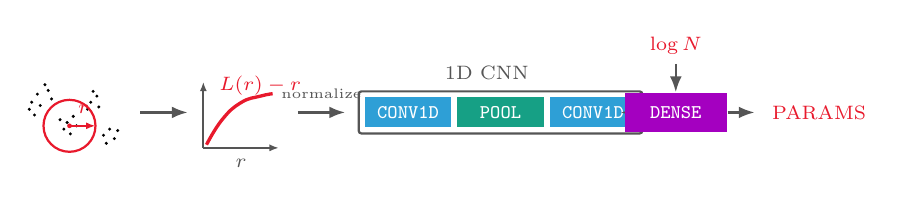
\begin{tikzpicture}
 \begin{scope}[shift={(0,0)},scale=0.6]
  \pointcloud{(0,0)}
  \draw[cred,thick] (1.0,0.55) circle (0.55);
  \fill[cred] (1.0,0.55) circle (0.05);
  \draw[cred,thick,-{Latex[length=1.2mm]}] (1.0,0.55) -- (1.55,0.55);
  \node[tens,anchor=south] at (1.3,0.60) {$r$};
 \end{scope}
 \draw[arr] (1.5,0.5) -- (2.1,0.5);
 \begin{scope}[shift={(2.3,0.05)},scale=0.8]
  \draw[cgray,thick,-{Latex[length=1.2mm]}] (0,0) -- (1.2,0);
  \draw[cgray,thick,-{Latex[length=1.2mm]}] (0,0) -- (0,1.05);
  \draw[cred,very thick] plot[smooth,tension=0.8]
    coordinates {(0.05,0.05) (0.3,0.45) (0.6,0.72) (0.9,0.82) (1.1,0.86)};
  \node[note,anchor=north] at (0.6,-0.02) {$r$};
  \node[tens,anchor=west] at (0.1,0.98) {$L(r)-r$};
 \end{scope}
 \draw[arr] (3.5,0.5) -- (4.1,0.5);
 \node[note,anchor=south,font=\tiny] at (3.8,0.55) {normalize};
 \node[conv,minimum width=1.1cm,minimum height=0.38cm] (v1) at (4.9,0.5) {CONV1D};
 \node[pool,minimum width=1.1cm,minimum height=0.38cm,right=0.06cm of v1] (v2) {POOL};
 \node[conv,minimum width=1.1cm,minimum height=0.38cm,right=0.06cm of v2] (v3) {CONV1D};
 \node[box,fit=(v1)(v3)] (vbox) {};
 \node[note,anchor=south] at (5.9,0.80) {1D CNN};
 \draw[arr] (vbox.east) -- (7.6,0.5);
 \node[lin,minimum width=1.3cm,minimum height=0.5cm] (dense) at (8.3,0.5) {DENSE};
 \node[tens] (logn) at (8.3,1.35) {$\log N$};
 \draw[arr] (logn.south) -- (dense.north);
 \draw[arr] (dense.east) -- (9.3,0.5);
 \node[tens,anchor=west] at (9.4,0.5) {PARAMS};
\end{tikzpicture}
\end{adjustbox}
\end{frame}

% -----------------------------------------------------------------------------
\begin{frame}{Vectorization methods}
\begin{figure}
  
\includegraphics[width=0.88\textwidth]{vectorization_schematic.pdf}
\end{figure}
\vspace{-6pt}
{\footnotesize
\begin{itemize}\setlength\itemsep{1pt}
  \item A filtration $\{F_r\}$ grows a family of complexes with parameter $r$;
        features ($H_0$ components, $H_1$ loops) are born and die, giving a
        diagram of pairs $(b,d)$.
  \item Diagrams are not Hilbert-space elements, so they must be vectorized
        before using in an ML pipeline.
  \item Many vectorizations have been proposed: images (Adams et al., 2017),
        Betti curves (Umeda, 2017), landscapes (Bubenik, 2015), silhouettes
        (Chazal et al., 2014).
  \item \alert{No formalized comparison exists in this setting}: Yip et al.\
        (2025) fix persistence images and vary only the homology dimension.
        This has been the central question of the project.
\end{itemize}}
\end{frame}

% -----------------------------------------------------------------------------
\begin{frame}{Choice of filtration}
\begin{center}
  
\includegraphics[width=0.55\textwidth]{dtm_vs_rips.pdf}
\end{center}
\vspace{-4pt}
{\footnotesize
\begin{itemize}\setlength\itemsep{2pt}
  \item \textbf{Rips} uses inter-point distances alone: it merges the two blobs
        through the sparse bridge. \textbf{$\DTM_k$} uses each point's RMS
        distance to its $k$ nearest neighbours, so a simplex enters according to
        how \emph{densely} its neighbourhood is occupied, so the merge is
        delayed.
  \item Point-process parameters act directly on local density, so $\DTM$ is a
        natural choice.
  \item Contrast with $K$, $g$: radial statistics collapse the cloud to a curve
        indexed by $r$, discarding \emph{how} density is distributed in space.
\end{itemize}}
\end{frame}

% -----------------------------------------------------------------------------
\begin{frame}{From point cloud to persistence images}
\begin{fitpicS}
 \pointcloud{(0,0.8)}
 \draw[cgray,thick] (-0.15,0.65) rectangle (2.25,2.45);
 \draw[arr] (2.4,1.6) -- (2.9,2.55);
 \draw[arr] (2.4,1.6) -- (2.9,0.65);
 \node[tens] (d1) at (3.55,2.6) {DTM($m_1$)};
 \node[note] at (3.55,1.6) {$\vdots$};
 \node[tens] (dk) at (3.55,0.6) {DTM($m_K$)};
 \draw[arr] (d1.east) -- ++(0.5,0);
 \draw[arr] (dk.east) -- ++(0.5,0);
 \pdplot{(4.75,2.1)}
 \pdplot{(4.75,0.1)}
 \node[note] at (5.3,1.6) {$\vdots$};
 \draw[arr] (5.95,2.6) -- (6.35,2.6);
 \draw[arr] (5.95,0.6) -- (6.35,0.6);
 \pigrid{(6.5,2.1)}{H0}
 \pigrid{(7.7,2.1)}{H1}
 \pigrid{(6.5,0.1)}{H0}
 \pigrid{(7.7,0.1)}{H1}
 \node[note] at (7.0,1.6) {$\vdots$};
 \node[note] at (8.2,1.6) {$\vdots$};
 \draw[arr] (8.9,1.6) -- (9.5,1.6);
 \node[tens,anchor=west] at (9.6,1.75) {$(B,\,K,\,2,\,64,\,64)$};
\end{fitpicS}
\vfill
{\color{cgray}\scriptsize
\begin{itemize}\setlength\itemsep{0.1em}
\item Add point on scales: only one used for Thomas and three for Nested. Defer full explanation to later. Mention that, individually, they are monotonic
 \item $64\times 64$ raster, fixed kernel width, exact per-pixel integration
\end{itemize}}
\end{frame}

% -----------------------------------------------------------------------------
\begin{frame}{ParamNet: CoordConv PI encoder + head}
\begin{fitpicS}
 \pigrid{(0,1.0)}{H0}
 \pigrid{(1.2,1.0)}{H1}
 \node[tens,anchor=north] at (1.1,0.85) {$(2,\,64,\,64)$};
 \node[note,anchor=north] at (1.1,0.40) {one DTM scale};
 \draw[arr] (2.5,1.5) -- (3.6,1.5);
 \node[note,align=center,anchor=south] at (3.05,1.6) {$+2$ coord\\ channels};
 \encoderstack{e}{(5.0,2.9)}
 \node[note,anchor=west] at (6.2,3) {$4 \to 32 \to 64 \to 128$};
 \node[note,anchor=west] at (6.2,0.30) {$128 \to 64$};
 \draw[arr] (6.1,1.5) -- (7.4,1.5);
 \node[tens,anchor=west] at (7.5,1.50) {$\R^{64}$ EMBEDDING};
 \node[tens] (logn) at (8.6,2.65) {$\log N(\pc)$};
 \draw[arr] (8.6,2.45) -- (8.6,1.65);
 \draw[arr] (9.9,1.5) -- (10.6,1.5);
 \headstack{h}{(11.6,2.4)}
 \node[note,anchor=south] at (11.6,2.75) {HEAD};
 \draw[arr] (11.6,0.2) -- (11.6,-0.35);
 \node[tens,anchor=north] at (11.6,-0.45) {PARAM ESTIMATE};
\end{fitpicS}
\vfill
{\color{cgray}\scriptsize
\begin{itemize}\setlength\itemsep{0.1em}
 \item Three $3{\times}3$ CoordConv blocks, widths $(32,64,128)$, ReLU,
       $2{\times}2$ max-pool, Dropout2d between blocks; adaptive average pool;
       linear to $\R^{64}$.
 \item A persistence image's axes are not arbitrary: birth encodes local
       density, persistence encodes separation. Absolute pixel position is
       informative, which is why I use CoordConv (see ablations).
 \item Head: hidden widths $64,32$ (ReLU, dropout $0.1$).
       AdamW, lr $10^{-3}$, weight decay $3\times10^{-4}$, batch size 32.
\end{itemize}}
\end{frame}

% -----------------------------------------------------------------------------
\begin{frame}{Simulator and design distribution}
\textbf{Naive sampling fails.} Uniform, independent draws per parameter put most
mass on near-Poisson or degenerate configurations.
\vspace{4pt}

\textbf{Reparameterize} according to properties of interest:
\[
\lambda = \kappa\mu, \qquad \kappa, \qquad \nu = r\sqrt{\kappa},
\qquad r = \sigma \ \text{(Thomas)}, \quad
r = \sqrt{\sigma_1^2+\sigma_2^2} \ \text{(nested)} .
\]
Draw $(\log\kappa,\log\lambda,\log\nu)$ uniformly and invert.
\vspace{4pt}

{\footnotesize
\begin{enumerate}\setlength\itemsep{2pt}
  \item \emph{Point budget}: $\lambda \in [150,800]$ --- persistence cost grows
        rapidly in $n$.
  \item \emph{Clusters per window}: $\kappa \in [15,120]$ --- enough to be
        informative, few enough to resolve.
  \item \emph{Overlap}: $\nu \in [0.10, 0.90]$ --- upper limit admits the
        weakly identifiable near-Poisson regime.
\end{enumerate}
}
\end{frame}

% -----------------------------------------------------------------------------

\begin{frame}{The near-Poisson regime}
\begin{center}
  
\includegraphics[width=0.78\textwidth]{regime_grid.pdf}
\end{center}
\vspace{2pt}
{\footnotesize
Simulated realisations across the overlap index
$\nu = r\sqrt{\kappa}$ at fixed $\lambda$, $\kappa$: Thomas (top) vs.\ nested
Thomas (bottom). $\nu \ll 1$: clusters countable, $\kappa$ easy to recover.\\
$\nu \gtrsim 1$: clusters merge, and many $(\kappa,\mu)$ pairs with the same
$\lambda$ give the same observable pattern.}
\end{frame}

% -----------------------------------------------------------------------------
\begin{frame}{Calibration of PIs}
\begin{columns}[T,onlytextwidth]
\begin{column}{0.44\textwidth}
  
\includegraphics[width=\textwidth]{calibration_comparison.pdf}
\end{column}
\begin{column}{0.52\textwidth}\footnotesize
\textbf{Problem.} For each pixel to mean the same thing, all diagrams need
shared axis ranges. Pooled min/max is stretched by a single outlier diagram, so
every other diagram is crushed toward the origin at fixed $64\times64$
resolution.
\vspace{6pt}

\textbf{Fix: per-diagram coverage quantiles.} With $b_i^{\min}, b_i^{\max},
p_i^{\max}$ computed \emph{within} each diagram,
\[
\bigl[\,Q_{1-q}(b^{\min}),\; \alpha\,Q_q(b^{\max})\,\bigr], \quad
\bigl[\,0,\; \alpha\,Q_q(p^{\max})\,\bigr]
\]
with $q = 0.95$, $\alpha = 1.05$, $\sigma_{\text{px}} = 0.5$, $G = 64$.
\vspace{6pt}

Ranges are fit on \emph{training} diagrams only, then frozen. Otherwise
held-out clouds leak into the training images.
\end{column}
\end{columns}
\end{frame}

% -----------------------------------------------------------------------------
\begin{frame}{Fusing $K$ scales: four variants}
\begin{fitpicS}
 \node[tens] (in) at (0.7,1.5) {$(K,\,2,\,64,\,64)$};
 \draw[arr] (1.8,1.5) -- (2.5,1.5);
 \encoderstack{e}{(3.5,2.9)}
 \node[note,anchor=south] at (3.5,3.25) {SHARED ENCODER};
 \draw[arr] (4.6,1.5) -- (5.3,1.5);
 \node[tens] (emb) at (6.1,1.5) {$(K,\,64)$};
 \draw[arr] (6.9,1.5) -- (7.6,1.5);
 \node[tens,align=center] (flat) at (8.7,1.5) {$(K\!\cdot\!64,\,)$};
 \node[note,anchor=south,align=center] at (8.7,1.85) {CONCAT\\ (order-blind)};
 \draw[arr] (9.8,1.5) -- (10.5,1.5);
 \headstack{h}{(11.5,2.4)}
 \node[note,anchor=south] at (11.5,2.75) {HEAD};
 \draw[arr] (11.5,0.2) -- (11.5,-0.35);
 \node[tens,anchor=north] at (11.5,-0.45) {PARAMS};
\end{fitpicS}
\vspace{-2pt}
\begin{center}
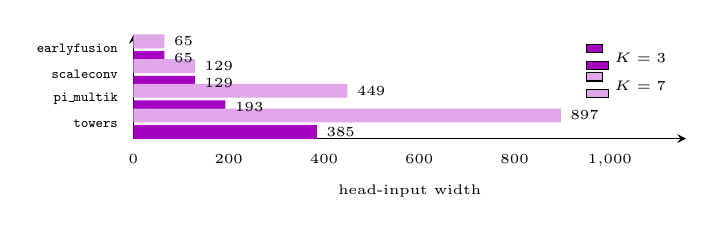
\begin{tikzpicture}
\begin{axis}[barlegend,
  xbar, width=8.6cm, height=2.9cm,
  bar width=5pt,
  xmin=0, xmax=1160,
  xlabel={\tiny head-input width},
  ytick={0,1,2,3},
  yticklabels={{\ttfamily towers},{\ttfamily pi\_multik},{\ttfamily scaleconv},{\ttfamily earlyfusion}},
  yticklabel style={font=\tiny},
  xticklabel style={font=\tiny},
  ymin=-0.6, ymax=3.6, enlarge y limits=false,
  nodes near coords, nodes near coords style={font=\tiny},
  axis lines=left, tick style={draw=none},
  legend style={draw=none,fill=none,font=\tiny,at={(0.99,0.97)},anchor=north east},
]
\addplot[fill=cpurple,draw=none,bar shift=-3pt] coordinates {(385,0) (193,1) (129,2) (65,3)};
\addplot[fill=cpurple!35,draw=none,bar shift=3pt] coordinates {(897,0) (449,1) (129,2) (65,3)};
\legend{$K=3$,$K=7$}
\end{axis}
\end{tikzpicture}
\end{center}
\vspace{-4pt}
{\color{cgray}\scriptsize
Variants differ \emph{only} in how the $K$ embeddings are fused. Only
\texttt{scaleconv} and \texttt{earlyfusion} keep a fixed head width as scales
are added.}
\end{frame}

% -----------------------------------------------------------------------------
\begin{frame}{Which scales carry the most signal?}
\begin{columns}[T,onlytextwidth]
\begin{column}{0.47\textwidth}
\centering
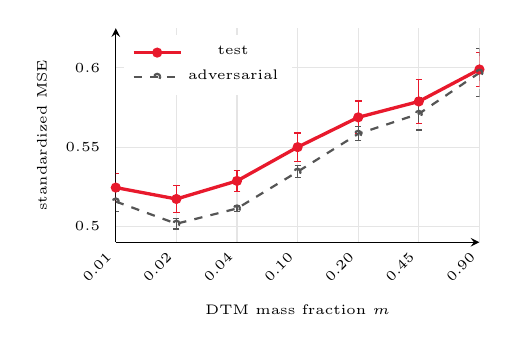
\begin{tikzpicture}
\begin{axis}[
  width=6.2cm, height=4.3cm,
  xtick={1,2,3,4,5,6,7},
  xticklabels={0.01,0.02,0.04,0.10,0.20,0.45,0.90},
  xlabel={\tiny DTM mass fraction $m$},
  ylabel={\tiny standardized MSE},
  xticklabel style={font=\tiny,rotate=45,anchor=east}, yticklabel style={font=\tiny},
  ymin=0.49, ymax=0.625,
  axis lines=left, tick style={draw=none},
  grid=major, grid style={gray!20},
  legend style={draw=none,font=\tiny,at={(0.02,0.97)},anchor=north west},
]
\addplot[cred,very thick,mark=*,mark size=1.2pt,
  error bars/.cd, y dir=both, y explicit]
 coordinates {(1,0.5245) +- (0,0.0091)
              (2,0.5173) +- (0,0.0083)
              (3,0.5287) +- (0,0.0067)
              (4,0.5500) +- (0,0.0089)
              (5,0.5688) +- (0,0.0103)
              (6,0.5788) +- (0,0.0141)
              (7,0.5990) +- (0,0.0108)};
\addplot[cgray,thick,dashed,mark=o,mark size=1.1pt,
  error bars/.cd, y dir=both, y explicit]
 coordinates {(1,0.5157) +- (0,0.0063)
              (2,0.5017) +- (0,0.0033)
              (3,0.5113) +- (0,0.0018)
              (4,0.5345) +- (0,0.0039)
              (5,0.5584) +- (0,0.0044)
              (6,0.5710) +- (0,0.0102)
              (7,0.5969) +- (0,0.0151)};
\legend{test,adversarial}
\end{axis}
\end{tikzpicture}\\
{\color{cgray}\tiny Single scale, $n=3$ seeds. Best: $m=0.02$.}
\end{column}
\begin{column}{0.51\textwidth}
\centering
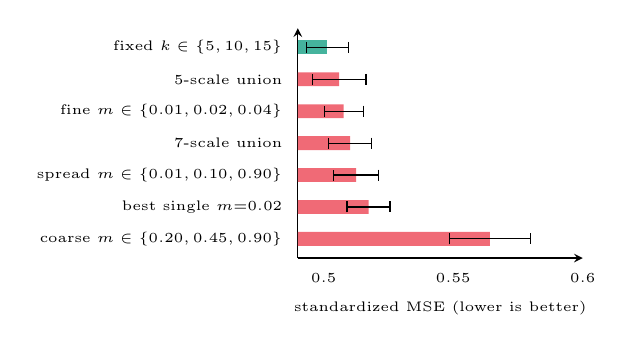
\begin{tikzpicture}
\begin{axis}[
  xbar, width=5.2cm, height=4.5cm, bar width=5pt,
  xmin=0.49, xmax=0.60,
  ytick={0,1,2,3,4,5,6},
  yticklabels={{coarse $m\in\{0.20,0.45,0.90\}$},
               {best single $m{=}0.02$},
               {spread $m\in\{0.01,0.10,0.90\}$},
               {7-scale union},
               {fine $m\in\{0.01,0.02,0.04\}$},
               {5-scale union},
               {fixed $k\in\{5,10,15\}$}},
  yticklabel style={font=\tiny}, xticklabel style={font=\tiny},
  xlabel={\tiny standardized MSE (lower is better)},
  ymin=-0.6, ymax=6.6, enlarge y limits=false,
  axis lines=left, tick style={draw=none},
]
\addplot[fill=cred!65,draw=none,bar shift=0pt,
  error bars/.cd, x dir=both, x explicit]
 coordinates {(0.5641,0) +- (0.0157,0)
              (0.5173,1) +- (0.0083,0)
              (0.5125,2) +- (0.0088,0)
              (0.5102,3) +- (0.0083,0)
              (0.5077,4) +- (0.0075,0)
              (0.5059,5) +- (0.0104,0)};
\addplot[fill=cgood!80,draw=none,bar shift=0pt,
  error bars/.cd, x dir=both, x explicit]
 coordinates {(0.5014,6) +- (0.0082,0)};
\end{axis}
\end{tikzpicture}\\
{\color{cgray}\tiny Every union containing a fine scale lands in
$0.506$--$0.513$; coarse-only is clearly worse; fixed $k$ best overall.}
\end{column}
\end{columns}
\end{frame}

% -----------------------------------------------------------------------------
\begin{frame}{Ablations}
\centering\scriptsize
\begin{tabular}{llcc}
\toprule
Axis & Arm & Thomas $\Loss$ & Nested-Thomas $\Loss$ \\
\midrule
Filtration    & Rips (vec\_multik, landscape) & $0.178 \pm 0.008$ & $0.461 \pm 0.016$ \\
              & $\DTM_5$ / $\DTM_{15}$ & $0.125 \pm 0.007$ / $0.146 \pm 0.006$ & $0.205 \pm 0.003$ / $0.260 \pm 0.017$ \\
              & $\DTM_{\{5,10,15\}}$ (fused) & $0.126 \pm 0.008$ & $0.192 \pm 0.010$ \\
Homology      & $H_0$ only / $H_1$ only & $0.125 \pm 0.006$ / $0.900 \pm 0.019$ & $0.280 \pm 0.250^{\dagger}$ / $0.932 \pm 0.028$ \\
Encoder       & shared / independent & $0.125 \pm 0.007$ / $0.134 \pm 0.009$ & $0.201 \pm 0.010$ / $0.222 \pm 0.021$ \\
Vectorization & Persistence image & $0.126 \pm 0.008$ & $0.192 \pm 0.010$ \\
              & Landscape & $0.132 \pm 0.008$ & $0.250 \pm 0.005$ \\
              & Silhouette ($p=1$) & $0.165 \pm 0.013$ & $0.271 \pm 0.012$ \\
              & Betti curve & $0.196 \pm 0.014$ & $0.290 \pm 0.005$ \\
Features      & $\log N$ removed & $0.217 \pm 0.278^{\dagger}$ & $0.203 \pm 0.007$ \\
              & Topology removed ($\log N$ only) & $0.893 \pm 0.015$ & $0.948 \pm 0.019$ \\
\bottomrule
\end{tabular}
\vspace{8pt}

\raggedright\footnotesize
\begin{enumerate}\setlength\itemsep{2pt}
  \item \textbf{The filtration matters.} Rips is the worst arm on both
        processes, and by a wide margin on nested Thomas
        ($0.461$ vs $0.192$).
  \item \textbf{$H_0$ carries the signal.} $H_0$ alone matches the full model;
        $H_1$ alone collapses to chance on both processes. Nested Thomas benefits from using both $H_0$ and $H_1$, Thomas does not.
  \item \textbf{The signal is in the images, not the point count.} $\log N$
        alone is at chance, while removing $\log N$ costs little.
\end{enumerate}
\vspace{2pt}
{\color{cgray}\scriptsize $n=10$ seeds per arm. $^{\dagger}$ at least one seed
failed to converge and collapsed to chance, so the mean is dominated by the
failed seed(s).}
\end{frame}

% -----------------------------------------------------------------------------
\begin{frame}{Benchmarking}
\centering\footnotesize
\begin{tabular}{lcc}
\toprule
Method & Thomas $\Loss$ & Nested $\Loss$ \\
\midrule
ParamNet$^{\ddagger}$     & $0.125 \pm 0.007$~{\scriptsize(26\%)}      & $\mathbf{0.192 \pm 0.010}$~{\scriptsize(27\%)} \\
\texttt{vihrs} ($L(r)-r$) & $\mathbf{0.115 \pm 0.007}$~{\scriptsize(25\%)} & $0.217 \pm 0.006$~{\scriptsize(29\%)} \\
Min.\ contrast, $K$       & $0.855 \pm 0.682^{a}$~{\scriptsize(83\%)}  & $179.12 \pm 150.33$~{\scriptsize($\sim\!1.4{\times}10^{5}$\%)} \\
Min.\ contrast, $g$       & $6.199 \pm 0.339^{b}$~{\scriptsize(407\%)} & $14.81 \pm 0.21$~{\scriptsize(701\%)} \\
\midrule
\emph{Chance (shuffle)}   & \emph{$1.003$}~{\scriptsize(92\%)}         & \emph{$1.006$}~{\scriptsize(72\%)} \\
\bottomrule
\end{tabular}

\vspace{4pt}
{\raggedright\scriptsize
$^{\ddagger}$process-specific: $\DTM_5$ / fused $\DTM_{5,10,15}$.
$^{a}$unstable across seeds rather than uniformly bad.
$^{b}$consistently worse than chance.\par}

\vspace{8pt}
\hrule
\vspace{5pt}

{\raggedright\footnotesize
\textbf{\texttt{vihrs} wins on Thomas}, on every parameter
($\Loss^\kappa\,0.192$, $\Loss^\mu\,0.122$, $\Loss^\sigma\,0.029$ vs
$0.201$, $0.134$, $0.040$): on a single-level process the topological pipeline
does not beat a hand-built radial summary.
\textbf{On nested Thomas} ParamNet gains on the density and count targets, while
\texttt{vihrs} still wins both scale parameters --- $L(r)-r$ is built to resolve
a characteristic radius, a density-based feature is not.
\vspace{4pt}

\textbf{Minimum contrast} fails for two different reasons. On $K$, 6/10 seeds
land close to \texttt{vihrs} and 4/10 blow up: the near-Poisson flatness. On
$g$, every seed is worse than chance --- systematic bias rather than scattered
non-convergence, likely my untuned contrast exponent $c=1$ where $c=1/4$ is the
value validated for aggregated patterns. I report the number but do not read it
as a claim about contrast estimation on $g$ in general.\par}
\end{frame}

% -----------------------------------------------------------------------------
\begin{frame}{Difficulty ordering}
\begin{columns}[T,onlytextwidth]
\begin{column}{0.62\textwidth}
  
\includegraphics[width=\textwidth]{paramnet_scatter.pdf}
\end{column}
\begin{column}{0.34\textwidth}\footnotesize
For \emph{every} method, on \emph{both} processes, parent intensity $\kappa$ is the hardest target and cluster scale $\sigma$ the
easiest.
\vspace{6pt}

Since the ordering survives changes of feature set \emph{and} architecture, it
looks like a property of the estimation problem rather than an artifact of any
one pipeline.
\end{column}
\end{columns}
\end{frame}

% -----------------------------------------------------------------------------
\begin{frame}{Limitations and planned directions}
\begin{columns}[T,onlytextwidth]
\begin{column}{0.48\textwidth}
\textbf{Limitations}\\[3pt]
{\footnotesize
\begin{itemize}\setlength\itemsep{1.5pt}
  \item \textbf{The process must be known.} ParamNet is trained on
        synthetic clouds, so it presumes the family is already identified
        and that a simulator exists for it.
        A practitioner holding one real pattern has neither: misidentify the
        family and the estimates are wrong.
  \item \textbf{Per-process choices.} The number and choice of filtration scales
        has no rule beyond validation-loss comparison, which undercuts the
        process-agnostic objective.
  \item \textbf{Comparison is architecture-bound.} Three alternative
        vectorizations lost, but under \emph{this} encoder and \emph{this}
        design distribution.
  \item \textbf{Not highly competitive.} No advantage on Thomas, only slight advantage on Nested Thomas (admittedly a pathological example)
  \item \textbf{The design distribution is a prior}; its ranges must cover the
        intended application.
  \item \textbf{Cost.} Persistence scales badly in $n$; inference cost per cloud
        is unmeasured.
\end{itemize}}
\end{column}
\begin{column}{0.48\textwidth}
\textbf{Next Steps}\\[3pt]
{\footnotesize
\begin{itemize}\setlength\itemsep{1.5pt}
  \item \textbf{Encoder architecture.} A process-agnostic encoder, and a
        properly matched encoder per vectorization for a fair comparison.
  \item \textbf{More processes.} Inhomogeneous / non-stationary, where classical
        closed forms are least available. Compare with two-step procedure of
        Waagepetersen \& Guan.
  \item \textbf{Bypass the parameters.} The process parameter are
        not typically the final quantity of interest: they are an intermediate step
        toward properties we actually want. Yip et al.\ (2025)
        map persistence images of a halo catalogue straight to the cosmological
        parameters $(\Omega_m, \sigma_8)$, without estimating $(\kappa,\mu,\sigma)$.
  \item \textbf{Classification as a front end.} Add a step that first infers
        \emph{which} process generated the cloud, then routes it to the matching
        ParamNet. This directly addresses the first limitation: the family stops
        being an input the user must supply and becomes something the pipeline
        determines.
\end{itemize}}
\end{column}
\end{columns}
\end{frame}

% =============================================================================
\section{Part II --- Hessian spectra during grokking}
% =============================================================================

\begin{frame}{The Grokking Phenomenon}
\textbf{Grokking} (Power et al., 2022): near-perfect \emph{train} accuracy in
$\sim\!10^3$ steps, \emph{test} accuracy at chance for $10^4$--$10^5$ further
steps, then a sharp transition.
\vspace{6pt}
\begin{itemize}
  \item Whatever separates the memorizing phase from the generalizing one is
        \alert{not visible in the training loss}.
  \item Following Fort \& Scherlis (2019)
        and Ghorbani et al.\ (2019), I used the Hessian's eigenvalue spectrum to study the local geometry of the loss landscape.
  \item Early exploration on MNIST / FashionMNIST showed an apparent
        \emph{spectral collapse} near the transition. I moved to modular
        arithmetic following Gromov (2023), which is the more standard setting.
  \item As this was my first project, I implemented the approximation machinery
        directly rather than calling PyHessian.
\end{itemize}
\end{frame}

% -----------------------------------------------------------------------------
\begin{frame}{Setup: modular addition}
\begin{columns}[T,onlytextwidth]
\begin{column}{0.58\textwidth}
  \includegraphics[width=\textwidth]{wd_curve_phenomenon.pdf}
\end{column}
\begin{column}{0.38\textwidth}\footnotesize
Small decoder-only transformer on $a + b \bmod p$, $p = 91$; AdamW,
effectively full-batch, weight decay large enough to penalize the pure
memorization solution; 150{,}000 steps.
\vspace{6pt}

Train saturates almost immediately; test sits at chance ($1/91$) for roughly
three decades of steps, then rises sharply.
\vspace{6pt}

Two hyperparameters control onset, and both were swept:
weight decay $0.45 \to 1.0$ in steps of $0.05$ (10 seeds each), and
initialization scale $\alpha \in \{1, 8\}$.
\end{column}
\end{columns}
\end{frame}

% -----------------------------------------------------------------------------
\begin{frame}{Observables and stochastic Lanczos quadrature}
\begin{columns}[T,onlytextwidth]
\begin{column}{0.40\textwidth}
\textbf{Eight scalar summaries} of the spectrum of
$H = \nabla^2_\theta \Loss(\theta)$:
\footnotesize
\begin{enumerate}\setlength\itemsep{0pt}
  \item \texttt{top\_eig}
  \item \texttt{bulk\_edge}
  \item \texttt{n\_outliers}
  \item \texttt{trace}
  \item \texttt{spectral\_entropy}
  \item \texttt{effective\_rank}
  \item \texttt{negative\_mass}
  \item \texttt{conditioning}
\end{enumerate}
\end{column}
\begin{column}{0.56\textwidth}\footnotesize
Forming $H$ explicitly is infeasible for $10^3$--$10^7$ parameters.
\begin{enumerate}\setlength\itemsep{1pt}
  \item \textbf{HVPs.} Pearlmutter: $Hv = \nabla_\theta(g(\theta)^\top v)$ from
        two backward passes --- $H$ is only ever touched through $v \mapsto Hv$.
  \item \textbf{Lanczos.} For each probe $j=1,\dots,k$, run $m$ steps to get a
        tridiagonal $T^{(j)} \in \R^{m\times m}$.
  \item \textbf{Quadrature.} $T^{(j)} = U\Lambda U^\top$; Ritz values are nodes,
        $w_i^{(j)} = (U^{(j)}_{1i})^2$ are weights. Matches the first $2m-1$
        moments of the spectral measure seen by $v^{(j)}$.
  \item \textbf{Pool} over probes to get $\hat\mu$.
  \item \textbf{Observables} are functionals of $\hat\mu$, e.g.\
        $\widehat{\mathrm{tr}}\,H = n\!\int\! \lambda \, d\hat\mu$.
\end{enumerate}
\end{column}
\end{columns}
\end{frame}

% -----------------------------------------------------------------------------
\begin{frame}{Estimator validation}
\centering\footnotesize
\begin{tabular}{llcc}
\toprule
Observable & Governed by & Min.\ $m$ & Min.\ $k$ \\
\midrule
\texttt{trace} & $k$ (Monte Carlo, $\propto k^{-1/2}$) & irrelevant & $\geq 100$ \\
\texttt{top\_eig} & $m$ & $\geq 20$ & 1 \\
\texttt{negative\_mass} (margin-thresholded) & $m$ & $\geq 30$--$50$ & $\geq 30$ \\
\texttt{spectral\_entropy} / \texttt{effective\_rank} & $m$ & $\geq 20$--$30$ & $\geq 30$ \\
\texttt{bulk\_edge} / \texttt{conditioning} (post-fix) & $m$ & $\geq 75$--$100$ & not yet swept \\
\bottomrule
\end{tabular}
\vspace{8pt}

\raggedright
\begin{itemize}\footnotesize
  \item Every observable was checked against exact-reference fixtures with known
        ground-truth spectra --- small networks whose Hessian can be
        materialized in full.
  \item The observables do \emph{not} converge together.Each
        has its own requirement on depth $m$ and probe count $k$. Two definitions also turned out
        to be measuring artefacts of the estimator rather than the spectrum, and
        were corrected.
  \item Production defaults $m = k = 100$, set by the deepest-converging pair.
\end{itemize}
\end{frame}

% -----------------------------------------------------------------------------
\begin{frame}{Current results}
\begin{columns}[T,onlytextwidth]
\begin{column}{0.44\textwidth}
\centering
  \begin{adjustbox}{max width=\textwidth,max totalheight=0.36\textheight}
    \includegraphics{onset_vs_wd.pdf}
  \end{adjustbox}\\[4pt]
  \begin{adjustbox}{max width=\textwidth,max totalheight=0.36\textheight}
    \includegraphics{effective_rank_compare.pdf}
  \end{adjustbox}
\end{column}
\begin{column}{0.53\textwidth}\footnotesize
\textbf{Onset (top).} Onset falls $\sim\!3150 \to \sim\!1350$ steps as weight
decay rises $0.45 \to 1.0$. At wd $= 1.0$, $\alpha = 8$ roughly doubles the
delay ($\sim\!2890$ vs $\sim\!1350$).
\vspace{6pt}

\textbf{Spectrum (bottom).} \texttt{effective\_rank} tracks how many curvature
directions the loss landscape is actively using. It collapses $13.4\times$ at
wd $=0.6$ and $14.2\times$ at wd $=1$ --- two runs that differ in wd, onset
step, and checkpoint count, agreeing within 6\% on the size of the drop. Of
the eight tracked observables it is the only one that reproduces this way:
\texttt{top\_eig} rises in both but by very different amounts ($2.7\times$ vs
$16.1\times$), and \texttt{trace\_corr} disagrees in sign between runs.
Steps are aligned to each run's own onset so the two overlay.
\vspace{6pt}
\hrule
\vspace{5pt}

\textbf{What this is not.} $n = 1$ seed per condition, no error bars. Some
checkpoints flagged unreliable (train acc $< 0.9$: 5/66 at wd $=0.6$, 19/150
at wd $=1$). \texttt{trace\_corr} also fails an alternate-normalizer check and
is omitted. Read the collapse factors as order-of-magnitude agreement against
a noisy background, not a clean trend.

\end{column}
\end{columns}
\end{frame}

% =============================================================================
\begin{frame}{Summary and plan}
\begin{columns}[T,onlytextwidth]
\begin{column}{0.48\textwidth}
\textbf{Part I --- ParamNet}\\[3pt]
{\footnotesize
Persistence images are informative about Neyman--Scott parameters: roughly an
order of magnitude below the label-shuffle ceiling on both processes, with the
``Features'' arms locating that signal in the images rather than $\log N$.
They do \emph{not} universally beat a well-chosen radial summary --- the
advantage is confined to the two-level process and its density/count targets.}
\end{column}
\begin{column}{0.48\textwidth}
\textbf{Part II --- Hessian spectra}\\[3pt]
{\footnotesize
A validated SLQ estimator with two corrected defects and per-observable
convergence requirements; first evidence that \texttt{effective\_rank} collapse
aligns with the grokking onset across two weight-decay settings.}
\end{column}
\end{columns}
\vspace{8pt}
\textbf{Next 12 months}
\begin{itemize}\footnotesize
  \item \emph{Weighted toward ParamNet}: process-agnostic encoder;
        inhomogeneous / non-stationary processes; real data (BCI).
  \item \emph{Grokking}: same-wd multi-seed replication with flagged checkpoints
        held out; validate the estimator against a real trained network rather
        than synthetic fixtures.
\end{itemize}
\end{frame}

\begin{frame}[plain]
\centering\vfill
{\Large\bfseries Thank you --- questions?}\\[0.35cm]
{\color{cred}\rule{4cm}{1.2pt}}
\vfill
\end{frame}

% =============================================================================
\appendix
% =============================================================================

\begin{frame}{Backup: Hessian spectrum at initialisation}
\centering
\includegraphics[width=0.46\textwidth]{plot7_arch_symmetry_scatter.png}\hfill
\includegraphics[width=0.46\textwidth]{plot8_arch_eigencount_scatter.png}
\vspace{4pt}

\raggedright\footnotesize
Two-spirals MLP, sweep over $(L, W, \sigma, \text{seed})$.
\textbf{Extremal asymmetry} ($\lambda_{\max} > |\lambda_{\min}|$ for 87.2\% of
points) alongside \textbf{near-perfect bulk symmetry}
($n_+/n_- \in [0.997, 1.131]$). Explained by $H = G + F$: $F$ is Wigner-class
and symmetric; $G$ is PSD with $\mathrm{erank} \approx 3$, so it displaces a
handful of eigenvalues rightward and cannot tilt the bulk. Both effects are
independent of $\sigma$.
\end{frame}

\begin{frame}{Backup: after 100 optimization steps}
\centering
\includegraphics[width=0.46\textwidth]{step100_plot7_arch_symmetry_scatter.png}\hfill
\includegraphics[width=0.46\textwidth]{step100_plot8_arch_eigencount_scatter.png}
\vspace{4pt}

\raggedright\footnotesize
Mass on negatives $0.462 \to 0.222$; $n_+/n_- \; 1.00 \to 1.50$;
$\mathrm{erank}(H) \; 50 \to 27$ while $\mathrm{erank}(G)$ is nearly unchanged
($3.10 \to 3.26$) --- the change is in $F$, consistent with $H$ approaching the
PSD matrix $G$ as residuals shrink.
\end{frame}

\begin{frame}{Backup: eigendensity proof-of-concept}
\centering
\includegraphics[width=0.31\textwidth]{sigmoid_kappa_vs_epoch.png}\hfill
\includegraphics[width=0.31\textwidth]{relu_kappa_vs_epoch.png}\hfill
\includegraphics[width=0.31\textwidth]{tanh_kappa_vs_epoch.png}
\vspace{4pt}

\raggedright\footnotesize
$\lambda_{\max}/\lambda_{\min}$ during training for sigmoid, ReLU and tanh.
The original feasibility check: MNIST, $[784,128,10]$, Adam, snapshots every
10 epochs. Test accuracies within $0.5\%$ of each other
($0.9789$ / $0.9742$ / $0.9753$) while the spectra evolve visibly differently
--- the observation that motivated pursuing spectra as a diagnostic.
\end{frame}

\end{document}